\documentclass[a4paper]{amsart}

\usepackage{color}
\usepackage[colorlinks=true, citecolor=red]{hyperref}  %needs to come before amsrefs package to work with \cite{}*{}
\usepackage{amssymb,latexsym}
\usepackage[alphabetic]{amsrefs}
\usepackage[mathscr]{eucal}
\usepackage{pdfsync}
\usepackage{graphicx}
\usepackage{epstopdf}
\DeclareGraphicsRule{.tif}{png}{.png}{`convert #1 `dirname #1`/`basename #1 .tif`.png}
\usepackage[all]{xy}
\usepackage{titletoc}
%\usepackage{txfonts}   %  \fint  for integral average

%\usepackage{showkeys}  %options notref  notcite 

%\input{rgb.tex}

%\textcolor{DarkRed}{text in DarkRed}


\CompileMatrices

\theoremstyle{plain}
\newtheorem{theorem}{Theorem}[section]
\newtheorem{lemma}[theorem]{Lemma}
\newtheorem{proposition}[theorem]{Proposition}
\newtheorem{corollary}[theorem]{Corollary}

\theoremstyle{definition}
\newtheorem{definition}[theorem]{Definition}%[section]


\theoremstyle{remark}
\newtheorem{defn}[theorem]{Definition} 
\newtheorem{example}[theorem]{Example}
\newtheorem{remark}[theorem]{Remark}
\newtheorem{discussion}[theorem]{Discussion}

%\numberwithin{equation}{section}

%\newcommand{\abs}[1]{\lvert#1\rvert}

\DeclareMathOperator{\Lip}{Lip}
\DeclareMathOperator{\dist}{dist}
\DeclareMathOperator{\expected}{\mathbb{E}}
\DeclareMathOperator{\prb}{Prob}
\DeclareMathOperator{\spt}{spt}
\DeclareMathOperator{\lap}{\Delta}
\DeclareMathOperator{\Tr}{Tr}

\raggedbottom

%\addtolength{\textwidth}{2cm}
%\addtolength{\oddsidemargin}{-1cm}
%\addtolength{\evensidemargin}{-1cm} 
%\addtolength{\topmargin}{-1cm} 
%\addtolength{\textheight}{2cm}

 
%%% BEGIN DOCUMENT
\begin{document}


\section{Background}

The main thing aimed at here is to get a natural measure on $ V $-variable fractals which is preserved under an appropriate transfer operator, and which is  a Gibbs measure in an appropriate sense.

\bigskip The following uses a little of the notation from the Advances paper and notation from your handwritten notes.

 \bigskip We are working with weighted IFSs, such as 
\[
F = (f^F_1,f^F_2,f^F_3; w_1^F,w_2^F,w_3^F), \quad G = (f^G_1,\dots,f^G_6; w_1^G,\dots,w_6^G),
\]
where $ F$ and $ G $ correspond to $ SG(2) $ and $ SG(3) $, with weights which typically are $ w_i^F = (r_i^F )^ \alpha $ where $ r_i^F =\Lip f^F_i $, etc., and $ \alpha $  is to be found from a Ruelle-Perron-Frobenius type theorem which we need to know/show works in our context.

It seems the appropriate space consists of pairs
\[
\Omega_V^* \oslash \Sigma^V :=
\big( (\omega^{(1)},\dots, \omega^{(V)}),  (\sigma^{(1)},\dots, \sigma^{(V)})\big)
\]
where $ 
 (\omega^{(1)},\dots, \omega^{(V)}) $
 is a $ V $-variable $ V $-tuple and   $ \sigma^{(i)} \in \Sigma(\omega^{(i)})$.  
 
In order to define the transfer operator on functions it seems necessary to work with $ V $-tuples.  Note also that one needs a path (i.e.\ point) in each $ \omega^{(i)} $.  This also seems necessary --- working with an address $ a $ as in your handwritten notes does not seem to contain enough information. Think about what happens in the trivial case $ V=1 $ and just one IFS, which is the usual deterministic setting.

The transfer operator is then the natural one:
\begin{equation} \label{dft}
\begin{gathered} 
T \big( (\omega^{(1)},\dots, \omega^{(V)}),  (\sigma^{(1)},\dots, \sigma^{(V)}\big) \\
 =
\Big( \big(T_{\sigma^{(1)}_1}\omega^{(1)},\dots, T_{\sigma^{(V)}_1}\omega^{(1)}\big),
\big(T\sigma^{(1)}, \dots, T\sigma^{(V)}\big)\Big),
\end{gathered}
\end{equation} 
using your notation.    $ T $ does preserve the class defined above.

\medskip 
The definition of the transfer operator $ \mathcal{L} $ on functions needed a lot of thought for me.  The approach used by Patschke does not work --- the problem is that it does not lead to a natural transfer operator on functions  with good properties in the $ V $-variable case.

But what Patschke does is equivalent to the following idea in the random recursive case.

\medskip First note that in the deterministic case, 
\[
(\mathcal{L} h)(\sigma)  = \sum_i w_i h (i\sigma) = \sum_{\{\tau:T\tau=\sigma\}} w_{\tau_1} h(\tau).
\]
This can also be interpreted, at least in the case that the $  w_i $ are probabilities, as
\[
(\mathcal{L} h)(\sigma) = \mathbb{E} ^x h(X(\sigma) ), 
\]
where $ X $ is a random variable starting at $ \sigma $ and proceeding to $ i \sigma $ with probability~$ w_i $.


\bigskip
In the random recursive case, motivated by the above,  it seems natural to define 
\begin{equation} \label{dfL} 
(\mathcal{L} h)(\omega,\sigma) = 
\mathbb{E}_{\widetilde{\omega}} \sum_{i=1}^{N(\widetilde{\omega})}
\Big( w_i(\widetilde{\omega})\, h(\widetilde{\omega},i\sigma) \ \Big| \ T_i\widetilde{\omega} = \omega \Big).
\end{equation} 
In other words, we are integrating (weighting) with respect to those $  \widetilde{\omega} $ subject to the conditional probability that at least one of the level one subtrees of  $  \widetilde{\omega} $ is the same as $ \omega $, and then weighting again with respect to the relevant  $ w_ i $.  

By using independence, this is equivalent to the form Patscheke uses, and he thus avoids using conditional probabilities.  (I should check this carefully).

But in the $ V $-variable case, \eqref{dfL} and the version used by Patschke  are not equivalent --- the $ V=1 $ case is an example.

%%%%%%%%%%%%%%%%%%%%%%%%%%%%
  \section{Transfer Operator on Functions}

 From \eqref{dft} and \eqref{dfL} one is led first to a natural definition for $ \mathcal{L}_V $ in the $ V=1 $ case and then for $ \mathcal{L}_V $ in the case of arbitrary $ V $. 
 
 To motivate this, consider Figure~\ref{figto}.
 
\begin{figure}[htbp] %  figure placement: here, top, bottom, or page
   \centering
   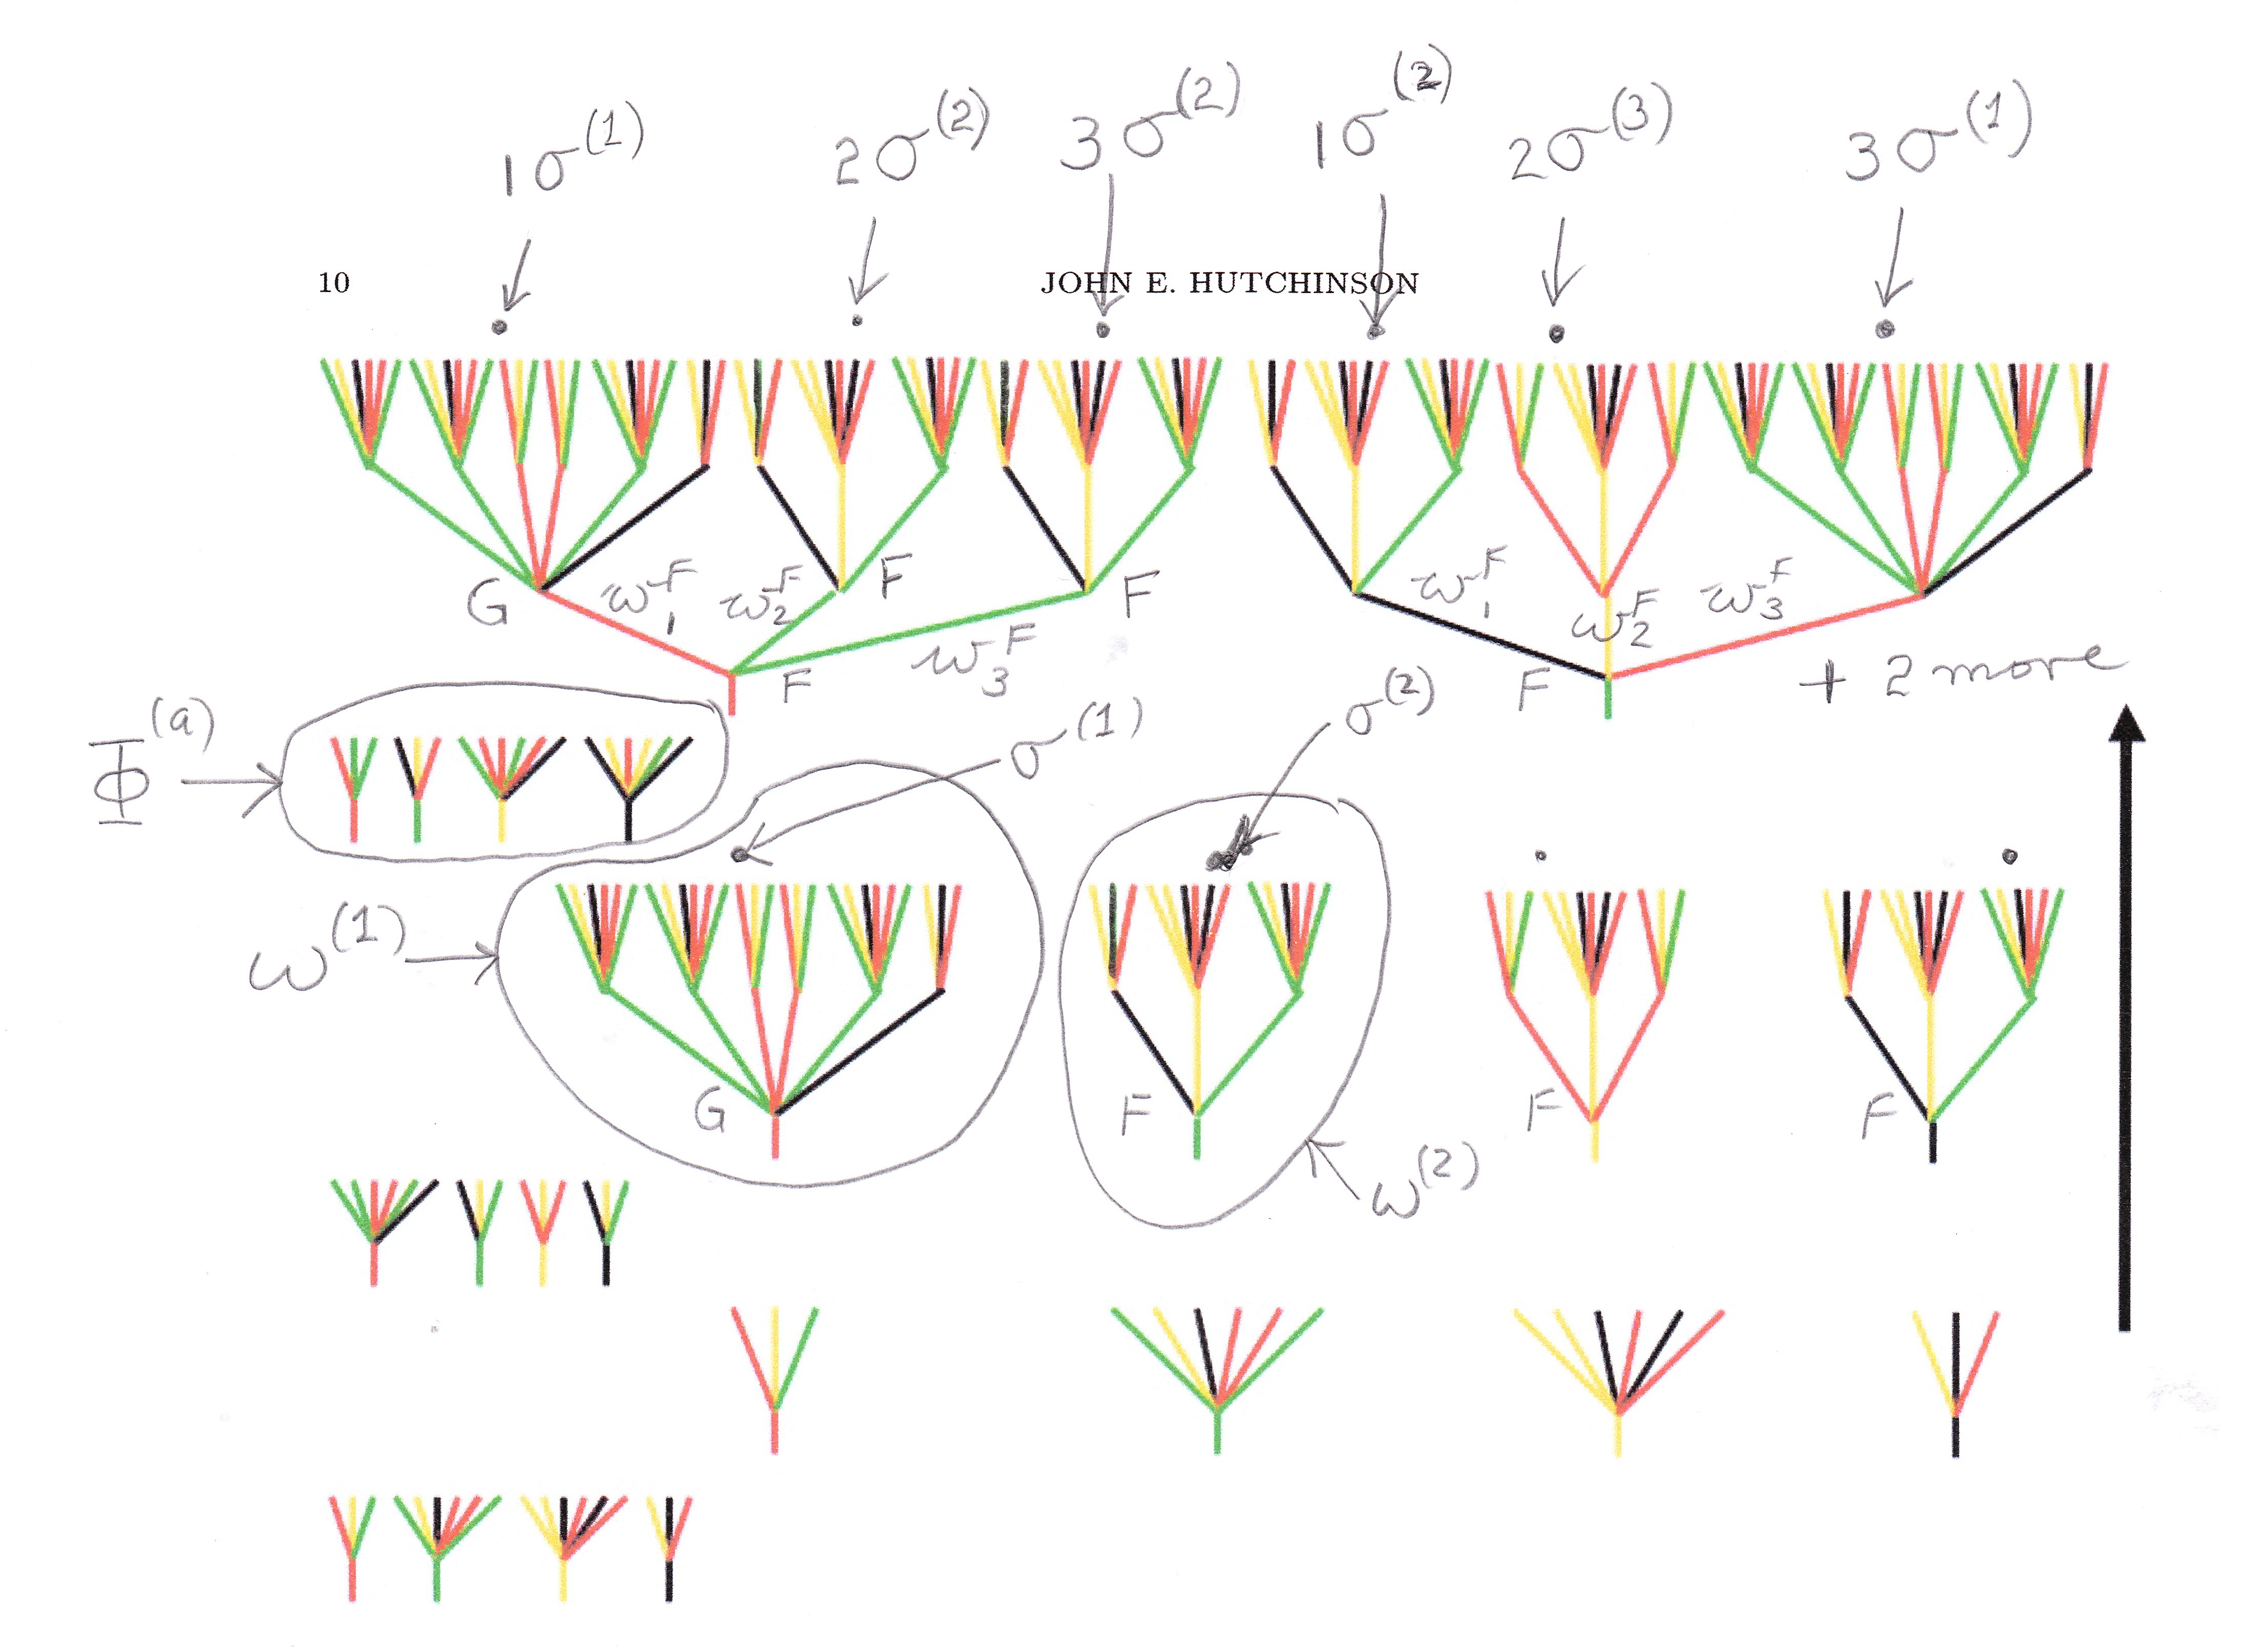
\includegraphics[width=5in]{IMG-2.jpg} 
   \caption{Transfer Operator} 
   \label{figto}
\end{figure}

 The third line from the top is $ (\omega^{(1)},\dots, \omega^{(4)})$ and the top line is
 \[
  (\widetilde{\omega}^{(1)},\dots, \widetilde{\omega}^{(4)}) = \Phi^a  (\omega^{(1)},\dots, \omega^{(4)}).
  \]
  An example of paths    $ \sigma^{(i)} $ is   shown in the third line from the top, and some of the paths $j \sigma^{(i)} $ are shown in the top line.
  
\medskip
The operator $ \Phi^a $ is given by the 4 small trees in the second line from the top.  In more standard notation,
\begin{equation} \label{}
\Phi^a = \begin{bmatrix}
  F & 1 & 2 & 2 & * & * & * \\
  F & 4 & 3 & 1 & * & * & * \\
 G & 2 & 1 & 1 & 2 & 1 & 4 \\
 G & 4 & 3 & 1 & 3  & 2 & 4 
 \end{bmatrix}
 \end{equation} 
For the box notation, see Figure~\ref{box}.	
\begin{figure}[htbp] %  figure placement: here, top, bottom, or page
   \centering
   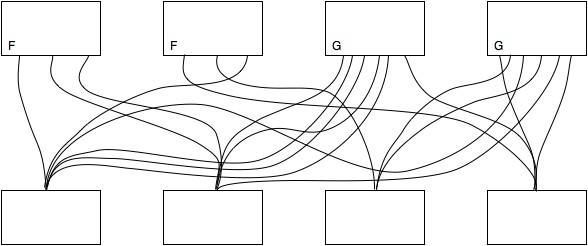
\includegraphics[width=5in]{box.jpg} 
   \caption{The bottom row of boxes contain  $  \omega^{(1)},\dots, \omega^{(4)}   $.  The operator $ \Phi^a $ is then applied to give $  \widetilde{\omega}^{(1)},\dots,   \widetilde{\omega}^{(4)}   $, which are placed in the top row of boxes.  The operator $   \Phi^a $ here is the same as in Figure~\ref{figto}.}
   \label{box}
\end{figure}

\bigskip
  In order to motivate the general definition of the transfer operator on functions, first consider the case $ V=1 $.  Then   $ a \in \mathcal{A}_V $ is completely described by choice of an IFS, and so in our test case with just two IFSs,  $ a $ corresponds to either $ F $ or $ G $.

In this test case suppose that the initial probability $ P $ on IFSs is given by $ P = \{p_F, p_G\} $. Then  \eqref{dfL} is equivalent  to the definition (this needs explanation)
\[
(\mathcal{L}_1 h)(\omega, \sigma) 
=  p_F \sum_{i=1}^3 w_i^F h(F  (\omega), i \sigma ) +  
p_G \sum_{i=1}^6 w_i^G h(G  (\omega), i \sigma ).
\]
In the general $ V=1 $ case (needs similar explanation)
\begin{align*} 
(\mathcal{L}_1 h)(\omega, \sigma) 
&= \int \bigg(  \sum_{i\in N(F^ \lambda )}  w_i^\lambda  h(F^ \lambda   (\omega), i \sigma ) \bigg) dP(\lambda ) \\
&= \int \bigg(  \sum_{i\in N( I(a)  )}  w_i^{I(a)}  h(\Phi^ a   (\omega), i \sigma ) \bigg) dP_1(a ),
\end{align*}
where $ N(F^ \lambda ) $ is the number of functions in the IFS $ F^ \lambda $ and $ N(I^a)$ is the number of functions  in the IFS $ F^{I^a}$ corresponding to $ a $.
  Note that $ \Phi^a $ corresponds to a single IFS $ F^ \lambda  $, and conversely.  The initial probability $ P $ on $  \Lambda $ is the same as the probability $ P_1 $ on $  \mathcal{A} _1 $.


\bigskip Now consider the  case for general $ V $.  We define a transfer operator acting on on functions
$ h: \Omega_V^*\oslash \Sigma^* \to \mathbb{R} $.



For $ a \in \mathcal{A}_V $ let 
\[
\Gamma^a = \{1,\dots, N(I^a(1))\} \times \dots \times \{1,\dots, N(I^a(V))\}
\]
index the set of ``allowable'' $ V $-tuples   of level one branches.
In Figure~\ref{box} this means  
\[
\Gamma^a = \{1,2,3\}\times \{1,2,3\}\times \{1,\dots, 6\} \times \{1,\dots,6\}.
\]
 
For $ \gamma     \in \Gamma^a $ let 
\[
w_ \gamma ^a = w_{\gamma(1)}^{I^a(1)} \times  \dots \times w_{\gamma(V)}^{I^a(V)}
\]
be the corresponding product of weights.  Note that if   the $ w_i^F $ are probabilities then 
$ \sum_{\gamma \in \Gamma^a} w_ \gamma ^a = 1 $.

Now once again, \eqref{dfL} is here equivalent (this needs explanation) to the following definition 
\begin{gather} \label{}
(\mathcal{L}_Vh) \Big( \big(\omega^{(1)},\dots, \omega^{(V)}\big),  
\big(\sigma^{(1)},\dots, \sigma^{(V)}\big)\Big) =\\
\int \bigg( 
\sum_{\gamma^a \in \Gamma^a} w_ \gamma ^a \,
     h \Big( \big( (\Phi^a\omega)^{(1)},\dots,  (\Phi^a\omega)^{(V)}\big),
                                      \big(\gamma^a (1) \sigma^{(1)},\dots, \gamma^a (V)\sigma^{(V)}\big) \Big)
\bigg) dP_V(a).\notag
\end{gather}

%%%%%%%%%%%%%%%%%%%%%%%%%%%%%%%%%
\section{What is Needed Next}
\begin{enumerate}

\item Write down the dual operator on measures in a reasonable notation

\item  Prove a Ruelle-Perron-Frobenius theorem, (and it may even follow directly from the standard one by defining a transformation on the appropriate space)

\item Prove a disintegration result

\item Hence get the required measure on a.e.\  $ V $-variable fractal
\end{enumerate} 




\end{document} 
 
 
 
 
 
 From \eqref{dft} and \eqref{dfL} one is led first to a natural definition in the $ V=1 $ case for $ \mathcal{L}_V $ and then for general $ V $.  I have to work out a decent notation, but the idea perhaps is clearer from the attached diagram.

The transfer operator acts on $ V $-tuples of functions to give another $ V $-tuple.  In the diagram with the $ \omega^{(i)} $ on the second line from the top and the $ \widetilde{\omega}^{(i)} $ on the top line, using an abuse of notation to pretend $ \mathcal{L}_V $ operates on single functions, one has
\begin{align*}
(\mathcal{L}_Vh) (\omega^{(1)},\sigma^{(1)}) &= w_1^Fh(\widetilde{\omega}^{(1)},1\sigma^{(1)}) 
  + w_3^Fh(\widetilde{\omega}^{(2)},3\sigma^{(1)}) \\
  &\quad + \text{ possible other terms from $ \widetilde{\omega}^{(3)}$ 
  and $ \widetilde{\omega}^{(4)} $}\\
  (\mathcal{L}_Vh) (\omega^{(2)},\sigma^{(2)}) &= w_2^Fh(\widetilde{\omega}^{(1)},2\sigma^{(2)}) 
  + w_2^Fh(\widetilde{\omega}^{(1)},3\sigma^{(2)}) 
   + w_1^Fh(\widetilde{\omega}^{(2)},1\sigma^{(2)})\\
  &\quad + \text{ possible other terms from $ \widetilde{\omega}^{(3)}$ 
  and $ \widetilde{\omega}^{(4)} $}
  \end{align*}  
\emph{However}, this is not really true.  One needs to integrate the expressions on the right according to the probability $ P_V $ on $ \mathcal{A}_V $.


 

